\setdictum{%
  B-splines are not enough!%
}{%
  In a talk at the 2017 SIAM Conference on\\
  Computational Science and Engineering%
}
% SIAM CSE 2017, Minisymposium MS154 "Flooding the Cores--Computing Flooding
% Events on Modern Architecture--Part I of II",
% Craig Michoski, UT Austin,
% "Scaling at Exascale in Blended Isogeometric, Discontinuous
% Galerkin, and Particle-in-Cell Approaches"

\chapter{Hierarchical B-Splines}
\label{chap:30BSplines}



\lettrine{I}{n} the last chapter,
we repeated the definition of sparse grids for
arbitrary tensor product basis functions.
The piecewise linear ``hat function'' basis $\varphi_{l,i}^1$
served as the motivation to omit hierarchical subspaces with
little contribution to the overall approximation quality.
However, the hat function basis is not continuously differentiable.
This has two implications.

\todo{mention order of splines on SGs?}

The first implication is that the approximation order of hat functions
is lower than the order of other basis function types
such as higher-degree splines \cite{Sickel11Spline}
or the piecewise polynomial basis by Bungartz \cite{Bungartz98Finite}.
The second implication, which also applies to Bungartz's basis,
is that we cannot compute globally continuous gradients of the
interpolant of a smooth objective function,
if we use non-smooth basis functions.
However, the availability of gradients is
essential in the application of gradient-based optimization,
which we target in this thesis.
In this chapter, we therefore define a hierarchical and
higher-order B-spline basis
(generalizing the well-known hat functions)
to obtain both higher-order approximations
as well as continuous gradients and Hessians.

The first to study B-splines was Isaac Schoenberg in 1946
\cite{Schoenberg46Contributions},
but he claimed that they had already been known to Laplace
\cite{Boor76Splines}.
Research and industry recognized the possibilities of B-splines when
the \fem, which is still the most significant application of B-splines,
emerged in the 1960s.
Carl de~Boor pioneered B-splines, developed basic algorithms, and
proved fundamental theoretical results \cite{Boor72Calculating}.
Researchers have applied B-splines in a diverse set of fields such as
\fem \cite{Hoellig03Finite} and \iga \cite{Hoellig12Finite},
geometric modeling with \nurbs
\multicite{Cohen01Geometric,Hoellig13Approximation},
financial mathematics \cite{Pflueger10Spatially},
molecular and atomic physics
\multicite{Bachau01Applications,McCurdy04Implementation},
and numerous other scientific and industrial areas.

In this chapter, we define hierarchical B-splines on sparse grids.
The chapter is divided into two sections:
First, we define hierarchical B-splines for both
uniform and non-uniform knot sequences in \cref{sec:31standardBSplines}.
Second, we learn in \cref{sec:32notAKnot} that the boundary behavior
of the classical uniform B-spline basis is problematic.
Incorporating not-a-knot boundary conditions into the B-spline basis
mitigates the problems caused by the boundary behavior.

\Cref{sec:311uniform} is a repetition of the definition
of nodal B-splines \multicite{Hoellig03Finite,Hoellig13Approximation} and
hierarchical B-splines \multicite{Pflueger10Spatially,Valentin14Hierarchische}.
Original contributions of the thesis in this chapter are the proof of
the linear independence of hierarchical B-splines in
\cref{sec:312proofHierarchicalSplitting}
(improved version of \cite{Valentin14Hierarchische},
published in \cite{Valentin16Hierarchical}),
the modified hierarchical Clenshaw-Curtis B-splines in
\cref{sec:314nonUniform} and
the hierarchical not-a-knot B-spline basis in \cref{sec:32notAKnot}.
\todo{add citation if Vazipfl has been published}



\section{Uniform and Non-Uniform Hierarchical B-Splines}
\label{sec:31standardBSplines}

\minitoc{83mm}{7}

\noindent
In this section, we mainly follow the presentation of
\multicite{Pflueger10Spatially,Valentin14Hierarchische,Valentin16Hierarchical}
to define hierarchical B-splines
starting from the well-known nodal B-spline basis
\multicite{Hoellig03Finite,Hoellig13Approximation,Quak16About}.
Note that thanks to the groundwork laid in \cref{chap:20sparseGrids},
especially \thmref{lemma:tensorProductLinearIndependence} and
\thmref{prop:splittingUVToMV},
it suffices to study the univariate case
of all bases that will be defined in the rest of this thesis.
The multivariate case is treated canonically by tensor products.



\subsection{Uniform Hierarchical B-Splines}
\label{sec:311uniform}

\paragraph{Cardinal B-splines}

The \term{cardinal B-spline}
$\cardbspl{p}\colon \real \to \real$ of \term{degree} $p \in \natz$
is defined by
\begin{equation}
  \label{eq:cardinalBSpline}
  \cardbspl{p}(x)
  :=
  \begin{cases}
    \displaystyle\int_0^1 \cardbspl{p-1}(x - y) \diff{}y,&p \ge 1,\\
    \charfun{\hopint{0, 1}}(x),&p = 0,
  \end{cases}
\end{equation}
where $\charfun{\hopint{0, 1}}$ is the characteristic function of
the half-open unit interval $\hopint{0, 1}$
(see \cite{Hoellig13Approximation}).
The cardinal B-spline $\cardbspl{p}$ has the following properties
\cite{Hoellig03Finite},
which are shown in \cref{fig:cardinalBSplineProps}:

\begin{figure}
  \includegraphics{cardinalBSplineProps_1}%
  \caption[%
    Properties of cardinal B-splines%
  ]{%
    Eight properties of cardinal B-splines using the quadratic case
    $p = 2$ as an example.\\
    \lefthphantom{1.}{5.}\,
    $\cardbspl{p}$ is compactly supported on $\clint{0, p+1}$.\\
    \lefthphantom{2.}{5.}\,
    $\cardbspl{p}$ is symmetric and $0 \le \cardbspl{p} \le 1$.\\
    \lefthphantom{3.}{5.}\,
    $\cardbspl{p}$ is a weighted combination of
    $\cardbspl{p-1}$ \emph{\textcolor{C0}{(blue)}} and
    $\cardbspl{p-1}({\cdot} - 1)$ \emph{\textcolor{C1}{(red)}.}\\
    %where the coefficients \emph{(dashed)} are linear in $x$.\\
    \lefthphantom{4.}{5.}\,
    $\cardbspl{p}$ is a piecewise polynomial of degree $p$.\\
    \lefthphantom{5.}{5.}\,
    $\deriv{x}{\cardbspl{p}}$ \emph{(dashed)}
    is the difference of
    $\cardbspl{p-1}$ \emph{\textcolor{C0}{(blue)}} and
    $\cardbspl{p-1}({\cdot} - 1)$ \emph{\textcolor{C1}{(red)}.}\\
    \lefthphantom{6.}{5.}\,
    $\cardbspl{p}$ has unit integral.\\
    \lefthphantom{7.}{5.}\,
    $\cardbspl{p}$ is the convolution of
    $\cardbspl{p-1}$ \emph{\textcolor{C0}{(blue)}} and $\cardbspl{0}$.\\
    \lefthphantom{8.}{5.}\,
    Hat function \emph{\textcolor{C0}{(blue)}} and
    Gaussian function \emph{\textcolor{C1}{(red)}}
    are special cases of $\cardbspl{p}$.%
  }%
  \label{fig:cardinalBSplineProps}%
\end{figure}

\begin{enumerate}
  \item
  \emph{Compact support:}
  The support of $\cardbspl{p}$ is given by $\supp \cardbspl{p} = \clint{0, p + 1}$.
  
  \item
  \emph{Bounds and symmetry:}
  The cardinal B-spline $\cardbspl{p}$ is non-negative and bounded from above by one.
  It is symmetric with respect to $x = \tfrac{p+1}{2}$, i.e.,
  $\cardbspl{p}(x) = \cardbspl{p}(p + 1 - x)$.
  
  \item
  \emph{Recursion:}
  The cardinal B-spline $\cardbspl{p}$ ($p \ge 1$)
  satisfies the following recurrence relation
  (which can be used as an alternative definition):
  \begin{equation}
    \cardbspl{p}(x)
    = \frac{x}{p} \cardbspl{p-1}(x) + \frac{p+1-x}{p} \cardbspl{p-1}(x-1).
  \end{equation}
  
  \item
  \emph{Spline:}
  On every \term{knot interval} $\hopint{k, k+1}$ for $k = 0, \dotsc, p$,
  $\cardbspl{p}$ is a polynomial of degree~$p$, i.e.,
  $\cardbspl{p}$ is a spline of degree $p$ (piecewise polynomial).
  
  \item
  \emph{Derivative:}
  At the \term{knots} $k = 0, \dotsc, p + 1$,
  $\cardbspl{p}$ is $(p - 1)$ times continuously differentiable (if $p \ge 1$).
  The derivative can be computed by differentiating
  \eqref{eq:cardinalBSpline}:
  \begin{equation}
    \label{eq:cardinalBSplineDerivative}
    \deriv{x}{\cardbspl{p}}(x)
    = \cardbspl{p-1}(x) - \cardbspl{p-1}(x-1),\quad
    x \in \real.
  \end{equation}
  
  \item
  \emph{Integral}:
  The B-spline $\cardbspl{p}$ has unit integral, i.e.,
  $\int_{\real} \cardbspl{p}(x) \dx = 1$.
  %\vspace{-0.5em}
  %\begin{equation}
  %  \int_{\real} \cardbspl{p}(x) \dx = 1.
  %\end{equation}
  
  \item
  \emph{Convolution:}
  The integral in the definition of $\cardbspl{p}$
  is the convolution $\cardbspl{p-1} \convolution \cardbspl{0}$
  of the B-spline $\cardbspl{p-1}$
  of degree $p - 1$ with the B-spline $\cardbspl{0}$ of degree zero.
  
  \item
  \emph{Generalization:}
  As a special case, $\cardbspl{1}$ is a hat function interpolating the data
  $\{(k, \kronecker{k}{1}) \mid k \in \integer\}$.
  For $p \to \infty$, the normalized cardinal B-splines converge
  pointwise to the standard Gaussian function
  $\cardbspl{\infty}(x) := (2\pi)^{-1/2} \exp(-x^2/2)$ \cite{Unser92Asymptotic}:%
  \footnote{%
    This can also be seen as a consequence of the central limit theorem
    applied to uniformly distributed random variables.
    The pointwise convergence of the probability density functions
    can be proven from the convergence
    in distribution using a converse to Scheffé's theorem
    \cite{Boos85Converse}.%
  }
  \vspace{-0.5em}
  \begin{equation}
    \lim_{p \to \infty}
    c^p \cardbspl{p}(c^p x + \tfrac{p+1}{2})
    = \cardbspl{\infty}(x),\quad
    c^p := \sqrt{\frac{p+1}{12}},\quad
    x \in \real.
  \end{equation}
\end{enumerate}

The cardinal B-splines of the first degrees are shown in
\cref{fig:cardinalBSpline}.
Due to the convolution property,
cardinal B-splines of degree $p \ge 2$ are ``smoothed versions''
of the hat function.
This is shown in the flip book animation in the bottom left corner
of the even-numbered pages of this thesis.

\begin{figure}
  \includegraphics{cardinalBSpline_1}%
  \caption[%
    Cardinal B-splines%
  ]{%
    Cardinal B-splines $\cardbspl{p}$ up to quintic degree $p = 5$.%
  }%
  \label{fig:cardinalBSpline}%
\end{figure}

\paragraph{Definition of uniform hierarchical B-splines}

\usenotation{Ëp}
As for the hat functions in \cref{chap:20sparseGrids},
we can use the cardinal B-spline $\cardbspl{p}$ as a ``parent function'' to
define the uniform hierarchical B-spline
$\bspl{l,i}{p}\colon \clint{0, 1} \to \real$ of level~$l \in \natz$ and index
$i \in \hiset{l}$ via an affine parameter transformation
\cite{Pflueger10Spatially}:
\begin{equation}
  \label{eq:uniformHierarchicalBSplineUV}
  \bspl{l,i}{p}(x)
  := \cardbspl{p}(\tfrac{x}{\ms{l}} + \tfrac{p+1}{2} - i).
\end{equation}
The support of $\bspl{l,i}{p}$ is given
by $\supp \bspl{l,i}{p} = \clint{0, 1} \cap \clint{\gp{l,i-(p+1)/2}, \gp{l,i+(p+1)/2}}$.
The hat function basis $\bspl{l,i}{1}$ defined in
\eqref{eq:hatFunctionUV} is a special case of
\eqref{eq:uniformHierarchicalBSplineUV} for $p = 1$,
which allows us to use the same notation $\bspl{l,i}{p}$ for both.
Note that due to the \term{translation invariance} of $\bspl{l,i}{p}$
(i.e., the basis functions are the same up to scaling and translation),
it suffices to precompute and implement the polynomial pieces of $\cardbspl{p}$
to enable evaluations of all hierarchical B-splines
$\bspl{l,i}{p}$ ($l \in \natz$, $i \in \hiset{l}$).

\begin{figure}
  \subcaptionbox{%
    Nodal B-splines $\bspl{l,i}{p}$ ($i \in \hiset{l}$) and grid points $\gp{l,i}$
    \emph{(dots).}%
  }[67mm]{%
    \includegraphics{hierarchicalBasis_4}%
  }%
  \hfill%
  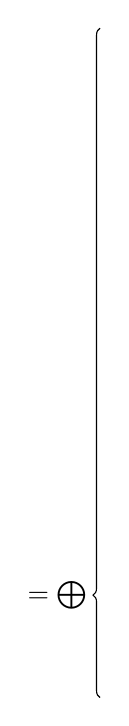
\begin{tikzpicture}
    \draw[decorate,decoration={brace,aspect=0.153}] (0,-8.5) -- (0,0);
    \node[anchor=east,inner sep=0mm] at (-0.15,-7.208) {$= \bigoplus$};
  \end{tikzpicture}%
  \hfill%
  \subcaptionbox{%
    Hierarchical B-splines $\bspl{l',i'}{p}$ ($l' \le l$, $i' \in \hiset{l'}$)
    and grid points $\gp{l',i'}$
    \emph{(dots).}%
  }[69mm]{%
    \includegraphics{hierarchicalBasis_5}%
  }%
  \caption[%
    Nodal and hierarchical B-splines%
  ]{%
    Univariate nodal and hierarchical cubic B-splines ($p = 3$)
    up to level $l = 3$.
    When restricting all functions to $\rspldomain{l}{p}$ \emph{(thick black line),}
    the nodal space $\restrictspace{\nsbspl{l}{p}}{\rspldomain{l}{p}}$ decomposes into the direct sum
    of the hierarchical subspaces $\restrictspace{\hsbspl{l'}{p}}{\rspldomain{l}{p}}$ ($l' \le l$).%
  }%
  \label{fig:hierarchicalBSpline}%
\end{figure}

\paragraph{Odd and even degrees}

In this thesis, we will only allow odd degrees $p = 1, 3, 5, \dotsc$
Many theoretical considerations fail for even degrees.
The basic reason is that for odd degrees, the knots of
$\bspl{l,i}{p}$ coincide with the grid points \cite{Valentin14Hierarchische}
\begin{equation}
  \gp{l,i-(p+1)/2},\quad
  \dotsc,\quad
  \gp{l,i},\quad
  \dotsc,\quad
  \gp{l,i+(p+1)/2}.
\end{equation}
For even degrees $p$, the knots of $\bspl{l,i}{p}$ lie exactly in
the middle between two subsequent grid points:
\begin{equation}
  \gp{l,i-p/2} - \frac{\ms{l}}{2},\quad
  \dotsc,\quad
  \gp{l,i} - \frac{\ms{l}}{2},\quad
  \gp{l,i} + \frac{\ms{l}}{2},\quad
  \dotsc,\quad
  \gp{l,i+p/2} + \frac{\ms{l}}{2}.
\end{equation}
This fact has many adverse implications on the hierarchical basis.
The most crucial implication is
that for even degrees $p$,
the hierarchical splitting \eqref{eq:hierSplittingUV} does not hold.
Furthermore,
we would not be able to define non-uniform hierarchical B-splines as
simple as for odd degrees and
fundamental splines would not be defined at all
(as we will see in \cref{sec:443fundamentalSplines}).
Additionally,
odd degrees include the hat function case~($p = 1$) and the
most commonly applied cubic degree~($p = 3$).
Therefore,
it is reasonable to restrict ourselves to odd degrees
for the rest of the thesis.



\subsection{Non-Uniform B-Splines and Proof of the Hierarchical Splitting}
\label{sec:312proofHierarchicalSplitting}

\paragraph{Non-uniform B-splines and spline space}

With the hierarchical B-splines $\bspl{l,i}{p}$, we can define
the nodal spaces $\nsbspl{l}{p}$ and hierarchical subspaces $\hsbspl{l}{p}$
as in \cref{chap:20sparseGrids}.
However, in order for the hierarchical splitting \eqref{eq:hierSplittingUV}
to be correct, we have to prove that the conditions of
\thmref{lemma:hierSplittingUV} are satisfied.
To investigate how the nodal space $\nsbspl{l}{p}$ looks like,
we introduce the notion of non-uniform B-splines.

\begin{definition}[non-uniform B-splines]
  \label{def:nonUniformBSpline}
  Let $m, p \in \natz$ and $\knotseq = (\knot{0}, \dotsc, \knot{m+p})$ be an
  increasing sequence of real numbers \term{(knot sequence).}
  For $k = 0, \dotsc, m - 1$,
  the \term{(non-uniform) B-spline} $\nonunifbspl{k,\knotseq}{p}$ of degree $p$
  with knots~$\knotseq$ and index $k$ is defined by the
  Cox--de~Boor recurrence
  \multicite{Cox72Numerical,Boor72Calculating,Hoellig13Approximation}
  \begin{equation}
    \nonunifbspl{k,\knotseq}{p}(x)
    :=
    \begin{cases}
      \dfrac{x - \knot{k}}{\knot{k+p} - \knot{k}} \nonunifbspl{k,\knotseq}{p-1}(x) +
      \dfrac{\knot{k+p+1} - x}{\knot{k+p+1} - \knot{k+1}}
      \nonunifbspl{k+1,\knotseq}{p-1}(x),&p \ge 1,\\
      \charfun{\hopint{\knot{k}, \knot{k+1}}}(x),&p = 0.
    \end{cases}
    \hspace*{-4mm}
  \end{equation}
\end{definition}
Note that when choosing $\knotseq = (0, 1, \dotsc, p + 1)$ and
$k = 0$, we obtain the cardinal B-spline~$\cardbspl{p}$.
\Cref{def:nonUniformBSpline} can be used to characterize
the nodal space $\nsbspl{l}{p}$:

\begin{proposition}[spline space]
  \label{prop:splineSpace}
  Let $\knotseq = (\knot{0}, \dotsc, \knot{m+p})$ be a knot sequence.
  Then, the B-splines $\nonunifbspl{k,\knotseq}{p}$ ($k = 0, \dotsc, m - 1$)
  form a basis of the \term{spline space}
  \begin{equation}
    \nonunifsplspace{\knotseq}{p}
    := \spn\{\nonunifbspl{k,\knotseq}{p} \mid k = 0, \dotsc, m - 1\}.
  \end{equation}
  $\nonunifsplspace{\knotseq}{p}$ contains exactly those functions that are continuous
  on $\spldomain{\knotseq}{p} := \clint{\knot{p}, \knot{m}}$,
  polynomials of degree $\le p$ on every knot interval
  $\hopint{\knot{k}, \knot{k+1}}$ in
  $\spldomain{\knotseq}{p}$
  ($k = p, \dotsc, m - 1$) and at least $(p - 1)$ times
  continuously differentiable at every knot $\knot{k}$ in the interior of
  $\spldomain{\knotseq}{p}$ ($k = p + 1, \dotsc, m - 1$).
\end{proposition}

\begin{proof}
  See \cite{Hoellig13Approximation}.
\end{proof}

This proposition gives the reason for the letter ``B'' in ``B-splines,''
which stands for ``basis'' (of the space of splines) \cite{Schoenberg67Spline}.
One example of a knot sequence and the corresponding B-splines is
given in \cref{fig:splineSpaceGeneral}.
The key observation is that B-splines of a knot sequence $\knotseq$
do not form a basis of the spline space on the union
$\clint{\knot{0}, \knot{m+p}}$ of the B-spline supports.
Instead, they form a basis of the spline space
on a proper sub-interval $\spldomain{\knotseq}{p}$.
Intuitively, for every point in $\spldomain{\knotseq}{p}$ that is not a knot,
exactly $p + 1$ B-splines must be \term{relevant} (non-zero)
to uniquely span the spline space,
as on every knot interval, the spline is a polynomial of degree $\le p$
and therefore, there must be $p + 1$ degrees of freedom.
Outside of $\spldomain{\knotseq}{p}$, there are too few relevant B-splines
to span the spline space.
This fact,
which is shown in \cref{fig:splineSpaceUniform},
forces us to restrict the nodal space and the hierarchical subspaces to
$\spldomain{\knotseq}{p}$:

\begin{figure}
  \includegraphics{splineSpace_1}%
  \caption[%
    Non-uniform B-splines with knot sequence and interpolation domain%
  ]{%
    Knot sequence $\knotseq = (\knot{0}, \dotsc, \knot{m+p}$)
    with the corresponding $m = 7$ non-uniform cubic B-splines
    $\nonunifbspl{k,\knotseq}{p}$ ($k = 0, \dotsc, m - 1$, $p = 3$).
    On $\spldomain{\knotseq}{p}$ \emph{(thick line, delimited by dashed lines),}
    which starts with the last knot interval of the first B-spline
    $\nonunifbspl{0,\knotseq}{p}$
    and ends with the first knot interval of the last B-spline
    $\nonunifbspl{m-1,\knotseq}{p}$,
    the B-splines span the spline space $\nonunifsplspace{\knotseq}{p}$.
    Elements of this space are splines $\spl\colon \spldomain{\knotseq}{p} \to \real$
    \emph{(black line),}
    which are linear combinations
    $\spl = \sum_{k=0}^{m-1} \interpcoeff{k} \nonunifbspl{k,\knotseq}{p}$
    of the B-splines.%
  }%
  \label{fig:splineSpaceGeneral}%
\end{figure}

\begin{figure}
  \includegraphics{splineSpace_2}%
  \caption[%
    Uniform nodal B-splines and knot sequence%
  ]{%
    Uniform knot sequence $\nodalknotseq{l}{p}$ \emph{(ticks on horizontal axis)}
    and corresponding nodal cubic B-splines ($p = 3$) of level $l = 3$.
    In the domain $\clint{0, 1}$ \emph{(delimited by dashed lines),}
    the grid points $\fgset{l}$ \emph{\textcolor{mittelblau}{(blue dots)}}
    coincide with the B-spline knots.
    The spline interpolation domain
    $\rspldomain{l}{p} := \spldomain{\nodalknotseq{l}{p}}{p}$
    \emph{(thick line)}
    is only a proper subset of $\clint{0, 1}$.%
  }%
  \label{fig:splineSpaceUniform}%
\end{figure}

\begin{corollary}[nodal B-spline space]
  \label{cor:nodalBSplineSpace}
  The restricted nodal B-splines $\restrictfcn{\bspl{l,i}{p}}{\rspldomain{l}{p}}$
  ($i = 0, \dotsc, 2^l$)
  of level $l \in \natz$ are
  a basis of the spline space $\nonunifsplspace{\nodalknotseq{l}{p}}{p}$,
  where
  \begin{subequations}
    \begin{gather}
      \nodalknot{l,k}{p}
      := (k - \tfrac{p+1}{2}) \ms{l},\quad
      k = 0, \dotsc, m + p,\quad
      m := 2^l + 1,\\
      \rspldomain{l}{p} := [\tfrac{p-1}{2} \ms{l},\;
      1 - \tfrac{p-1}{2} \ms{l}],
    \end{gather}
  \end{subequations}
  and consequently
  \begin{equation}
    \restrictspace{\nsbspl{l}{p}}{\rspldomain{l}{p}}
    = \restrictedsplspace{l}{p}
    := \nonunifsplspace{\nodalknotseq{l}{p}}{p}.
  \end{equation}
\end{corollary}

\begin{proof}
  We have $\bspl{l,i}{p} = \nonunifbspl{i,\nodalknotseq{l}{p}}{p}$ for
  $i = 0, \dotsc, m - 1$,
  as the B-splines on both sides have the same knots.
  The assertions now follow from \thmref{prop:splineSpace}.
\end{proof}

Note that $\rspldomain{l}{p}$ might contain only a single point or even be empty,
if $p$ is too large or $l$ is too small.
However, the corresponding B-splines $\bspl{l,i}{p}$ are still linearly
independent on~$\clint{0, 1}$ (see \cite{Hoellig13Approximation}).
Similarly, the corollary also implies that the hierarchical functions
$\bspl{l,i}{p}$ of level $l$ ($i \in \hiset{l}$)
are linearly independent on $\clint{0, 1}$.

\paragraph{Hierarchical splitting for uniform B-splines}

We can use \cref{prop:splineSpace} and \cref{cor:nodalBSplineSpace}
to prove the hierarchical splitting for the uniform B-spline basis
\cite{Valentin16Hierarchical}.

\begin{lemma}[hierarchical B-splines in nodal space]
  \label{lemma:hierBSplineInNodalSpace}
  The restricted hierarchical subspaces
  $\restrictspace{\hsbspl{l'}{p}}{\rspldomain{l}{p}}$ ($l' \le l$) are
  subspaces of the restricted nodal space $\restrictspace{\nsbspl{l}{p}}{\rspldomain{l}{p}}$.
\end{lemma}

\begin{proof}
  Every function $\bspl{l',i'}{p}$ ($i' \in \hiset{l'}$) is continuous on
  $\rspldomain{l}{p}$, a polynomial of degree $\le p$ on every knot interval
  of $\nodalknotseq{l}{p}$ (due to $p$ odd),
  and at the knots themselves at least $(p - 1)$ times continuously
  differentiable.
  \Cref{prop:splineSpace} implies $\bspl{l',i'}{p} \in \restrictedsplspace{l}{p}$
  and from \cref{cor:nodalBSplineSpace}, it follows
  $\bspl{l',i'}{p} \in \restrictspace{\nsbspl{l}{p}}{\rspldomain{l}{p}}$.
  As the functions $\bspl{l',i'}{p}$ ($i' \in \hiset{l'}$) span
  $\restrictspace{\hsbspl{l'}{p}}{\rspldomain{l}{p}}$, we can conclude
  $\restrictspace{\hsbspl{l'}{p}}{\rspldomain{l}{p}} \subset \restrictspace{\nsbspl{l}{p}}{\rspldomain{l}{p}}$.
\end{proof}

It is crucial to note that this lemma does not hold for even $p$,
as the knots of the B-splines of level $l - 1$ are not contained in the
knots of level $l$.
This implies that in general,
$\restrictspace{\hsbspl{l-1}{p}}{\rspldomain{l}{p}}$
is not contained in $\restrictspace{\nsbspl{l}{p}}{\rspldomain{l}{p}}$
for even degrees $p$.
Therefore, the hierarchical splitting equation \eqref{eq:hierSplittingUV}
does not hold.

\begin{restatable}[hierarchical B-splines are linearly independent]{%
  proposition%
}{%
  propHierBSplineLinearlyIndependent%
}
  \label{prop:hierBSplineLinearlyIndependent}
  The hierarchical B-splines
  $\bspl{l',i'}{p}$ ($l' \le l$, $i' \in \hiset{l'}$)
  are linearly independent.
\end{restatable}

\begin{proof}
  See \cref{sec:a121proofHierBSplineLinearlyIndependent}.
\end{proof}

Although we have to restrict all functions and spaces to $\rspldomain{l}{p}$,
\thmref{lemma:hierSplittingUV} is still applicable to prove that
the hierarchical splitting equation \eqref{eq:hierSplittingUV}
is correct for hierarchical B-splines:

\begin{corollary}[hierarchical splitting for uniform B-splines]
  \label{cor:hierSplittingBSpline}
  The hierarchical splitting \eqref{eq:hierSplittingUV}
  holds for the hierarchical B-spline basis
  if restricting all functions to $\rspldomain{l}{p}$:
  \begin{equation}
    \restrictedsplspace{l}{p}
    = \restrictspace{\nsbspl{l}{p}}{\rspldomain{l}{p}}
    = \bigoplus_{l'=0}^l \restrictspace{\hsbspl{l'}{p}}{\rspldomain{l}{p}}.
  \end{equation}
\end{corollary}

\begin{proof}
  Analogously to the proof of \thmref{lemma:hierSplittingUV}
  and apply \thmref{cor:nodalBSplineSpace}.
\end{proof}

This corollary is also visualized in \cref{fig:hierarchicalBSpline}.
We can now proceed to define
multivariate nodal spaces $\nsbspl{\*l}{p}$,
multivariate hierarchical subspaces $\hsbspl{\*l}{p}$, and
sparse grid spaces $\regsgspace[p]{n}{d}$ as in \cref{chap:20sparseGrids}.
Note that it is possible to choose different degrees $p_t$ for
different dimensions $t = 1, \dotsc, d$,
since the hierarchical splitting \eqref{eq:hierSplittingMV} does not
require the bases in each dimension to be the same.
Consequently, we can define degree-dimension-adaptive
(so-called \term{$hp$-adaptive}) sparse grids
$\regsgspace[\*p]{n}{d}$ for arbitrary odd degree vectors $\*p$.

In the course of this thesis, we will derive multiple variations
of the standard hierarchical B-spline basis.
We will not repeat formal proofs of the hierarchical splitting equation
\eqref{eq:hierSplittingUV}
(i.e., verifying the two conditions of \cref{lemma:hierSplittingUV})
for each of theses bases for the sake of brevity.
The idea of the proof of \cref{prop:hierBSplineLinearlyIndependent},
which is inductively exploiting the smoothness conditions given by
B-splines of previous levels, can be transferred to similar B-spline
bases.



\subsection{Modification}
\label{sec:313modification}

\paragraph{Marsden's identity}

Similar to the piecewise linear case in \cref{sec:242modified},
Pflüger defined modified
hierarchical B-splines to obtain reasonable values on the boundary
without having to place grid points there \cite{Pflueger10Spatially}.
The main motivation is to define basis
functions $\bspl[\modified]{l,i}{p}$ that satisfy natural boundary
conditions, i.e.,
\begin{equation}
  \label{eq:naturalBoundaryConditions}
  \deriv[2]{x}{\bspl[\modified]{l,i}{p}}(x) = 0,\quad
  x \in \bndrydomain{\clint{0, 1}} = \{0, 1\}.
\end{equation}
Originally, this requirement stems from financial problems
\cite{Pflueger10Spatially}.
For the left boundary,
\eqref{eq:naturalBoundaryConditions} can be satisfied by
modifying the left-most function $\bspl{l,1}{p}$ such that
$\bspl[\modified]{l,1}{p}(x) = 2 - \tfrac{x}{\ms{l}}$ is a linear polynomial
when $x$ is ``near'' the boundary.
As in \cite{Pflueger10Spatially},
we append $\bspl{l,1}{p}$ with
B-splines $\bspl{l,i}{p}$ with index $i \le 0$ and
use \term{Marsden's identity} to compute the corresponding coefficients.
The identity enables us to explicitly compute the B-spline coefficients
of an arbitrary polynomial of degree $\le p$ by giving an explicit formula
for the B-spline coefficients of shifted monomials $({\cdot} - y)^p$.
Interestingly, the coefficients are polynomials themselves (in $y$):

\vspace*{0pt plus 0.5fill}

\begin{lemma}[Marsden's identity]
  \label{lemma:marsden}
  Let $p \in \natz$ and
  $\knotseq = (\knot{0}, \dotsc, \knot{m+p})$ be a knot sequence.
  Then, for all $x \in \spldomain{\knotseq}{p}$ and $y \in \real$,
  \begin{equation}
    \label{eq:marsden}
    (x - y)^p
    = \sum_{k=0}^{m-1}
    \;\bracket*{(\knot{k+1} - y) \dotsm (\knot{k+p} - y)}\;
    \nonunifbspl{k,\knotseq}{p}(x).
  \end{equation}
\end{lemma}

\begin{proof}
  See \cite{Hoellig13Approximation}.
\end{proof}

\vspace*{0pt plus 1fill}

\paragraph{Modified hierarchical B-splines}

By extending the sum in Marsden's identity to $i \in \integer$ and
comparing the coefficients of $y^p$ and $y^{p-1}$ of both sides,
we obtain representations for the first two monomials:
\begin{equation}
  1
  = \sum_{i \in \integer} \bspl{l,i}{p}(x),\quad
  x
  = \sum_{i \in \integer} \gp{l,i} \bspl{l,i}{p}(x),\quad
  x \in \real.
\end{equation}
This can be used to derive a definition for $\bspl[\modified]{l,i}{p}$:
\begin{equation}
  \label{eq:modifiedBSplineConstruction}
  2 - \frac{x}{\ms{l}}
  = 2 \sum_{i \in \integer} \bspl{l,i}{p}(x)
  - \frac{1}{\ms{l}} \sum_{i \in \integer} \gp{l,i} \bspl{l,i}{p}(x)
  = \sum_{i \in \integer} (2 - i) \bspl{l,i}{p}(x),\quad
  x \in \real.
\end{equation}
Note that only the B-splines with $i \ge 1 - \tfrac{p+1}{2}$
are relevant for the unit interval
as all other B-splines vanish in $\clint{0, 1}$.
Pflüger omits summands with $i > 1$ as he only wants to modify
$\bspl{l,1}{p}$ left of its grid point $\gp{l,1}$ \cite{Pflueger10Spatially}.
The right-most function $\bspl[\modified]{l,2^l-1}{p}$ can be derived
analogously by mirroring $\bspl[\modified]{l,1}{p}$ at $x = \tfrac{1}{2}$.
\pagebreak%
For~$l = 1$, again the ``constant one'' function is taken for the definition
of modified hierarchical B-splines (see \cref{fig:modifiedBSpline}):
{%
  \setlength{\abovedisplayskip}{9pt}%
  \setlength{\belowdisplayskip}{9pt}%
  \begin{equation}
    \label{eq:modifiedBSplineDefinition}
    \bspl[\modified]{l,i}{p}(x)
    :=
    \begin{cases}
      1,&
      l = 1,\quad i = 1,\\
      \displaystyle\sum_{i'=1-(p+1)/2}^1\!\!\!\! (2 - i') \bspl{l,i'}{p}(x),&
      l \ge 2,\quad i = 1,\\
      \bspl{l,i}{p}(x),&
      l \ge 2,\quad i \in \hiset{l} \setminus \{1, 2^l - 1\},\\
      \bspl[\modified]{l,1}{p}(1 - x),&
      l \ge 2,\quad i = 2^l - 1.
    \end{cases}
  \end{equation}%
}%
By \thmref{prop:splineSpace},
this definition implies that
$\bspl{l,1}{p}(x) = 2 - \tfrac{x}{\ms{l}}$ ($l \ge 2$)
is only valid for $x \in \clint{0, \tfrac{5-p}{2} \ms{l}}$, i.e.,
the second derivative at $x = 0$ vanishes only for $p \le 5$.
For higher degrees, it is non-zero, albeit very small
in its absolute value.
To enforce natural boundary conditions
for higher than quintic degrees,
the upper bound of $i'$ in the sum in \eqref{eq:modifiedBSplineDefinition}
must be extended to $\tfrac{p+1}{2}$.
In addition, more than just the left-most and the right-most inner
hierarchical B-spline must be modified for $p \ge 5$,
as the size of the supports of $\bspl{l,i}{p}$ increases
for growing $p$.

\begin{figure}
  \subcaptionbox{%
    Construction of the modified hierarchical cubic B-spline
    $\bspl[\modified]{l',1}{p}$ (\emph{dashed,} $l' \ge 2$)
    as a linear combination of neighboring B-splines $\bspl{l',i'}{p}$.%
  }[72mm]{%
    \includegraphics{modifiedBSpline_1}%
  }%
  \hfill%
  \subcaptionbox{%
    Modified hierarchical cubic B-splines $\bspl[\modified]{l',i'}{p}$
    ($l' = 1, \dotsc, l$, $i' \in \hiset{l'}$) and grid points $\gp{l',i'}$
    \emph{(dots).}%
  }[72mm]{%
    \includegraphics{hierarchicalBasis_6}%
  }%
  \caption[%
    Modified hierarchical B-splines%
  ]{%
    Construction of modified hierarchical cubic B-splines ($p = 3$) and
    the resulting basis up to level $l = 3$.%
  }%
  \label{fig:modifiedBSpline}%
\end{figure}



\subsection{Non-Uniform Hierarchical B-Splines}
\label{sec:314nonUniform}

Sparse grid spaces and their corresponding grid point sets,
as we have defined them in \cref{chap:20sparseGrids},
are completely independent of the actual location of the grid points
$\gp{l,i}$.
Therefore, it is possible to use different distributions for the grid points
than the standard equidistant choice of $\gp{l,i} = i \cdot \ms{l}$,
if the basis functions are altered accordingly
\cite{Valentin14Hierarchische}.
\usenotation{Ëcc}
The so-called Chebyshev points $\ccgp{l,i}$ and the
resulting Clenshaw--Curtis grids and B-splines will serve as an example.

\paragraph{Chebyshev points and Clenshaw--Curtis grids}

The \term{Chebyshev points} $\ccgp{l,i}$ of level $l \in \natz$
are defined as
\begin{equation}
  \ccgp{l,i}
  := \frac{1 - \cos(\pi \gp{l,i})}{2},\quad
  i = 0, \dotsc, 2^l,
\end{equation}
see \cite{Xu16Chebyshev} for example.
Chebyshev points are the locations of the extrema%
\footnote{%
  The literature sometimes uses the name ``Chebyshev points'' for
  the roots of $T_{2^l}$, which are closely connected with the extrema.
  One way to distinguish them is to call the extrema
  ``Chebyshev--Lobatto points'' and the roots
  ``Chebyshev--Gauss points'' \cite{Xu16Chebyshev}.%
}
of the Chebyshev polynomials $T_{2^l}$, which are defined as
$T_{2^l}\colon \clint{0, 1} \to \real$,
$T_{2^l}(x) := \cos(2^l \arccos(2x - 1))$.
They are obtained
geometrically by dividing a semicircle into $2^l$ equally-sized
segments and subsequently orthogonally projecting the
segment endpoints onto the diameter
(see \cref{fig:pointSplittingChebyshev}).
Analytically, they are determined by minimizing
the interpolation error term in polynomial interpolation.
The most practical use of Chebyshev points is in
polynomial interpolation to avoid Runge's phenomenon and in
numerical integration (quadrature), resulting in the
so-called Clenshaw--Curtis quadrature rules.

\begin{SCfigure}
  \includegraphics{pointSplitting_2}%
  \caption[%
    Decomposition of the set of univariate Clenshaw--Curtis grid points%
  ]{%
    The set of Chebyshev points $\fgset[\cc]{l}$ of level
    $l = 4$ \emph{(top)}
    decomposes into hierarchical grids of level $l' \le l$
    (compare with \cref{fig:pointSplittingUniform}).
    The Chebyshev points are constructed as
    the orthogonal projection of the
    endpoints of $2^l$ equally-sized segments
    of a semicircle onto its diameter \emph{\textcolor{C8}{(gray, top)}.}%
  }%
  \label{fig:pointSplittingChebyshev}%
\end{SCfigure}

In some settings, it may be beneficial to use full or sparse grids consisting
of Chebyshev points, which are then called \term{Clenshaw--Curtis grids,}
instead of uniform grids.
Besides the already mentioned advantages for polynomials and
quadrature, Clenshaw--Curtis grids can help to reduce interpolation
errors in a neighborhood of the boundary of the domain due to the increased
grid point density near the boundary
(at the cost of a lower grid point density in the interior).
If we want to use Chebyshev points as grid points for sparse grids,
we have to employ an appropriate basis to ensure that interpolation
is still possible.

\paragraph{Hierarchical Clenshaw--Curtis B-splines}

The \term{hierarchical Clenshaw--Curtis B-spline}
$\bspl[\cc]{l,i}{p}$ of level $l \in \natz$ and index
$i \in \hiset{l}$ is defined as \cite{Valentin14Hierarchische}
\begin{equation}
  \bspl[\cc]{l,i}{p}
  := \nonunifbspl{i,\nodalknotseq[\cc]{l}{p}}{p},
\end{equation}
where
\begin{subequations}
  \label{eq:clenshawCurtisBSplineKnots}
  \begin{gather}
    \nodalknot[\cc]{l,k}{p}
    :=
    \begin{cases}
      (k - \frac{p+1}{2}) \cdot \ccgp{l,1},&
      k = 0, \dotsc, \frac{p-1}{2},\\
      \ccgp{l,k-(p+1)/2},&
      k = \frac{p+1}{2}, \dotsc, 2^l + \frac{p+1}{2},\\
      1 + (k - 2^l - \frac{p+1}{2}) \cdot \ccgp{l,1},&
      k = 2^l + \frac{p+3}{2}, \dotsc, 2^l + p + 1,
    \end{cases}\\
    k = 0, \dotsc, m + p,\quad
    m := 2^l + 1.
  \end{gather}
\end{subequations}
For the construction of the knot sequence $\nodalknotseq[\cc]{l}{p}$,
the Chebyshev points $\ccgp{l,i}$
are equidistantly extended onto the real line $\real$.
As for the standard hierarchical B-spline basis,
it is now straightforward to define nodal spaces
$\nsbspl[\cc]{l}{p}$
and hierarchical subspaces $\hsbspl[\cc]{l}{p}$ as well as
sparse grid spaces $\regsgspace[p,\cc]{n}{d}$ and
grid point sets $\regsgset[\cc]{n}{d}$
using tensor products of Clenshaw--Curtis B-splines
and Cartesian products of Chebyshev point sets.
The one-dimensional cubic Clenshaw--Curtis basis and a
sparse Clenshaw--Curtis grid are shown in \cref{fig:clenshawCurtis}.

\begin{figure}
  \subcaptionbox{%
    Hierarchical cubic Clenshaw--Curtis B-splines
    $\bspl[\cc]{l',i'}{p}$
    ($l' \le l$, $i' \in \hiset{l'}$, $p = 3$) and
    modified Clenshaw--Curtis B-splines
     $\bspl[\cc,\modified]{l',i'}{p}$
    \emph{(dashed).}%
  }[72mm]{%
    \includegraphics{hierarchicalBasis_7}%
  }%
  \hfill%
  \subcaptionbox{%
    Sparse Clenshaw--Curtis grid $\regsgset[\cc]{n}{d}$
    of level $n = 4$ in $d = 2$ dimensions.%
  }[72mm]{%
    \includegraphics{sg_7}%
  }%
  \caption[%
    Clenshaw--Curtis B-splines and sparse grids%
  ]{%
    Clenshaw--Curtis B-splines and sparse grids.%
  }%
  \label{fig:clenshawCurtis}%
\end{figure}

Note that Clenshaw--Curtis B-splines
$\bspl[\cc]{l,i}{p}$ are not translation-invariant,
in contrast to $\bspl{l,i}{p}$.
As a result, both implementation effort and computation time for evaluation
are significantly higher for Clenshaw--Curtis B-splines than
for the standard uniform basis,
as the Clenshaw--Curtis B-splines cannot be precomputed.

\paragraph{Modification and generalizations}

We define \term{modified hierarchical Clenshaw--Curtis B-splines}
$\bspl[\cc,\modified]{l,i}{p}$ using the
same method as in \eqref{eq:modifiedBSplineDefinition}.
Here, the second derivative of $\bspl[\cc,\modified]{l,1}{p}$
does not vanish at $x = 0$ even for degrees $p \le 5$,
as the formula \eqref{eq:modifiedBSplineConstruction}
derived from \thmref{lemma:marsden} assumes uniform knots.
However, since most of the B-spline knots in the summation formula
lie outside $\clint{0, 1}$ and are thus uniform according
to \eqref{eq:clenshawCurtisBSplineKnots},
the absolute deviation of the second derivative from zero is small.
Again, to enforce natural boundary conditions,
we can recompute the coefficients
of the components $\bspl[\cc]{l,i'}{p}$
dynamically with Marsden's identity using the correct Chebyshev knots
in \eqref{eq:marsden}.

Note that our framework permits arbitrary grid point distributions
$\gp{l,i}^\ast$,
as long as two requirements are met:
First, their number should grow exponentially
(i.e., there are $2^l + 1$ points $\gp{l,i}^\ast$ in each level $l \in \natz$),
and second, they should be nested
(i.e., \eqref{eq:rewriteGridPoint} holds).
Appropriate non-uniform B-spline bases can be defined analogously
to Clenshaw--Curtis B-splines.

\section{Boundary Behavior of Hierarchical B-Splines}
\label{sec:32notAKnot}

As we have seen in the last section (see \cref{cor:hierSplittingBSpline}),
the hierarchical splitting equation \eqref{eq:hierSplittingUV}
only holds when restricting the function spaces to
$D_l^p = \clint{\ms{l} \tfrac{p-1}{2},\; 1 - \ms{l} \tfrac{p-1}{2}}$,
which is for $p > 1$ a proper subset of the domain $\clint{0, 1}$.
The implications of this fact on the approximation quality
of the hierarchical B-spline basis are severe.
In this section, we study the underlying reasons of the restriction and
we introduce a new B-spline basis that does not suffer from this issue.



\subsection{Approximation Power of Uniform Hierarchical B-Splines}
\label{sec:321approximation}

\todo{add references to Vazipfl paper if published}

\paragraph{Interpolation of polynomials}

Splines are a piecewise generalization of polynomials.
Consequently, approximation spaces spanned by splines of degree $p$ should
at least contain all polynomials of degree $\le p$,
since the approximation power of splines should be at least as good
as that of polynomials.
Unfortunately, this statement is not true for the uniform B-splines
$\basis{l,i}^p$ as we have defined them in the last section.
A counterexample is given in \cref{fig:nakInterpolation},
in which a cubic polynomial $f$ is interpolated with
hierarchical cubic B-splines.
However, one can clearly deviations of the interpolant from the polynomial
near the boundary, where the relative error exceeds \SI{10}{\percent}.
The oscillations occur even in the interior of the
spline interpolation domain $D_l^p$.
Of course, this phenomenon does not improve the approximation quality
for other non-polynomial functions as well.

\begin{figure}
  \subcaptionbox{%
    Objective function \textcolor{C0}{$f$ \emph{(blue)}},
    interpolant \textcolor{C1}{$\tilde{f}$ \emph{(red, dashed)}},
    grid points \emph{(dots)}, and
    spline interpolation domain $D_3^p$ \emph{(thick line)}.%
  }[75mm]{%
    \includegraphics{nakInterpolation_1}%
  }%
  \hfill%
  \subcaptionbox{%
    Relative error $\abs{(f - \tilde{f})/f}$ on a logarithmic scale.%
  }[75mm]{%
    \includegraphics{nakInterpolation_2}%
  }%
  \caption{%
    Hierarchical cubic B-splines $\basis{l',i'}^p$
    ($l' \le l$, $i' \in \hiset{l'}$, $p = 3$)
    fail to interpolate the cubic polynomial
    $f(x) := -10.2 x^3 + 14.7 x^2 - 5x + 0.7$
    on the grid of level $l = 3$.%
  }
  \label{fig:nakInterpolation}
\end{figure}

We can explain this as follows:
According to \thmref{cor:hierSplittingBSpline},
we have $\restrictedsplspace{l}{p} = \bigoplus_{l'=0}^l \hs{l'}^p|_{D_l^p}$
with $p = 3$.
Since cubic polynomials as $f$ are cubic splines as well,
$f \in \restrictedsplspace{l}{p}$ and hence
$f \in \bigoplus_{l'=0}^l \hs{l'}^p|_{D_l^p}$.
This means that there is a linear combination of hierarchical B-splines
$\basis{l',i'}^p$ ($l' \le l$, $i' \in \hiset{l'}$)
that interpolates $f$ exactly on the whole domain $D_l^p$
(not be confused with $\tilde{f}$ in \cref{fig:nakInterpolation},
which does not interpolate $f$ exactly in $D_l^p$).
However, in general, this interpolant is not equal $f$ outside
of $D_l^p$ (i.e., in $\clint{0, 1} \setminus D_l^p$),
as \thmref{prop:splineSpace} only holds for $D_l^p$.
In particular, the interpolant evaluated at $x \in \{0, 1\}$ is not
equal to $f(x)$.
If we now force the additional interpolation conditions in
$\gp{l,0} = 0$ and $\gp{l,2^l} = 1$,
the resulting interpolant $\tilde{f}$ cannot be the same as the previous
interpolant,
which is why $f$ and $\tilde{f}$ differ inside $D_l^p$.

\paragraph{Schoenberg--Whitney conditions}

Formally, the unique existence of an interpolating spline is
described by the so-called Schoenberg--Whitney conditions:

\begin{proposition}[Schoenberg--Whitney conditions]
  Let $\knotseq = (\knot{0}, \dotsc, \knot{m+p})$ be a knot sequence
  and $t_0, \dotsc, t_{m-1}$ a sequence of interpolation points with
  $\knot{p} \le t_0 < \dotsb < t_{m-1} \le \knot{m}$.
  Then, there exists a unique interpolating spline
  $s = \sum_{k=0}^{m-1} \interpcoeff{k} \nonunifbspl{k,\knotseq}{p}$ for arbitrary data if and only if
  \begin{equation}
    \knot{k} < t_k < \knot{k+p+1},\quad
    k = 0, \dotsc, m - 1.
  \end{equation}
\end{proposition}

\begin{proof}
  See \cite{Hoellig13Approximation}.
\end{proof}

The Schoenberg--Whitney conditions require that the interpolation points
are contained in $D_l^p$.
In the example of $p = 3$ in \cref{fig:nakInterpolation},
the points $x = 0$ and $x = 1$ do not lie in~$D_l^p$.
For general degree $p$, the first $\tfrac{p-1}{2}$ and the
last $\tfrac{p-1}{2}$ grid points of level $l$ are missing from $D_l^p$,
thus violating the Schoenberg--Whitney conditions.
One possible remedy would be to move these interpolation points inside
$D_l^p$ without changing the corresponding basis functions
(i.e., the knots would stay the same) \cite{Hoellig13Approximation}.
For instance in the cubic case, we could move $x = 0$ and $x = 1$ to
$x = 1.5 \ms{l}$ and $x = 1 - 1.5 \ms{l}$, respectively.
However, with this approach, we would not be able to interpolate
boundary values.
In addition, the condition of the interpolation problem will most likely
worsen if we place interpolation points near the end of the supports
of the corresponding basis functions.

\paragraph{Restriction to spline subspaces}

As often, taking slightly a different view of the problem helps
to find a solution.
Let $\wholesplspace{l}{p}$ denote the space of all splines of degree $p$
on the grid of level $l$, i.e., the space $\nonunifsplspace{\knotseq}{p}$ with
\begin{equation}
  \label{eq:fullGridKnots}
  \knot{k} := (k - p) \ms{l},\quad
  k = 0, \dotsc, m + p,\quad
  m := 2^l + p.
\end{equation}
We have $D_\knotseq^p = \clint{0, 1}$ for this choice of $\knotseq$, i.e.,
the grid points $\gp{l,i}$ ($i = 0, \dotsc, 2^l$) satisfy
the Schoenberg--Whitney conditions for the uniform B-spline basis.
Clearly, the sum $\bigoplus_{l'=0}^l \hs{l}^p$ is a subspace of $\wholesplspace{l}{p}$,
but it cannot equal $\wholesplspace{l}{p}$ due to
\begin{equation}
  \dim \bigoplus_{l'=0}^l \hs{l}^p
  = 2^l + 1
  < 2^l + p
  = m
  = \dim \wholesplspace{l}{p},\quad
  p > 1,
\end{equation}
by \thmref{prop:splineSpace}.
There are too few nodal (and hierarchical) basis functions to
span the whole spline space $\wholesplspace{l}{p}$.

The key idea is now to impose additional $(p - 1)$ boundary conditions
on the basis functions to restrict $\wholesplspace{l}{p}$ to a reasonable subspace
with the correct dimension $(2^l + p) - (p - 1) = 2^l + 1$.
``Reasonable'' means that besides this dimension constraint,
two requirements should be met:
First, the Schoenberg-Whitney conditions should be satisfied for
the new subspace and the grid of level $l$.
Second, the new subspace should contain all polynomials of degree $\le p$,
eliminating the issue discussed in \cref{fig:nakInterpolation}
in the process.



\subsection{Hierarchical Not-A-Knot B-Splines}
\label{sec:322NAKBSplines}

\paragraph{Not-a-knot conditions}

A suitable subspace can be obtained by incorporating the
so-called \term{not-a-knot boundary conditions} into $\wholesplspace{l}{p}$.
For the cubic case $p = 2$,
for which we need two conditions,
the not-a-knot conditions demand that
$\frac{\diff^3}{\dx^3} s$ is continuous at the first and last
interior knot $\gp{l,1} = \ms{l}$ and $\gp{l,2^l-1} = 1 - \ms{l}$
for all splines $s$ in the subspace.
Equivalently, $\gp{l,1}$ and $\gp{l,2^l-1}$ are effectively removed from the
knot sequence (hence ``not-a-knot''),
as this is equivalent to requiring that
$s$ is a cubic polynomial on $\clint{0, \gp{l,2}}$ and $\clint{\gp{l,2^l-2}, 1}$.
For general degree $p$ (in which we need $(p - 1)$ conditions),
we require that the $p$-th derivative $\frac{\diff^p}{\dx^p} s$
is continuous at the first $\tfrac{p-1}{2}$ and the last $\tfrac{p-1}{2}$
inner grid points
\begin{equation}
  \label{eq:removedNAKKnots}
  \gp{l,i},\quad
  i \in \{1, \dotsc, \tfrac{p-1}{2}\} \cup
  \{2^l - \tfrac{p-1}{2}, \dotsc, 2^l - 1\},
\end{equation}
which is equivalent to removing these knots from the knot sequence $\knotseq$,
or, alternatively, to requiring that $s$ is a polynomial
of degree $\le p$ on $\clint{0, \gp{l,(p+1)/2}}$ and on $\clint{\gp{l,2^l-(p+1)/2}, 1}$.

\newgsymbol{.nak}{$\cdot^\notaknot$}{%
  Superscript for ``Not-a-knot (knot sequence/basis
  function/function space/interpolant)''%
}%
\newgsymbol{xilpnak}{$\nodalknotseq{l}{p}{\notaknot}$}{%
  Knot sequence
  for nodal not-a-knot B-splines of level $l$, degree $p$%
}%
The knot sequence $\nodalknotseq{l}{p}{\notaknot}$
with not-a-knot boundary conditions is defined as follows:
\begin{subequations}
  \begin{gather}
    \nodalknotseq{l}{p}{\notaknot}
    := (\nodalknot{l,0}{p}{\notaknot}, \dotsc,
    \nodalknot{l,m+p}{p}{\notaknot}),\quad
    m := 2^l + 1,\\
    \nodalknot{l,k}{p}{\notaknot}
    :=
    \begin{cases}
      \gp{l,k-p},&
      k = 0, \dotsc, p,\\
      \gp{l,k-(p+1)/2},&
      k = p + 1, \dotsc, 2^l,\\
      \gp{l,k-1},&
      k = 2^l + 1, \dotsc, 2^l + p + 1.
    \end{cases}
  \end{gather}
\end{subequations}
This knot sequence $\nodalknotseq{l}{p}{\notaknot}$
can be obtained by removing the knots
given in \eqref{eq:removedNAKKnots} from the
knot sequence \eqref{eq:fullGridKnots} for the full grid of level $l$.
The resulting spline space
\begin{equation}
  \naksplspace{l}{p}
  := \nonunifsplspace{\nodalknotseq{l}{p}{\notaknot}}{p}
\end{equation}
is a subspace
of $\wholesplspace{l}{p}$ with the correct dimensionality:
\begin{equation}
  \dim \bigoplus_{l'=0}^l \hs{l}^p
  = 2^l + 1
  = \dim \naksplspace{l}{p}.
\end{equation}
The new space $\naksplspace{l}{p}$ satisfies our two requirements:
First, the spline interpolation domain of $\naksplspace{l}{p}$
equals the whole interval.
This means that the Schoenberg--Whitney conditions are satisfied
for $\naksplspace{l}{p}$, since all interpolation points
(grid points) lie within $D_{\nodalknotseq{l}{p}{\notaknot}}^p = \clint{0, 1}$.
Second, $\naksplspace{l}{p}$ still contains all polynomials of
degree $\le p$, as we have only removed knots compared to $\wholesplspace{l}{p}$.

\begin{figure}
  \includegraphics{splineSpace_3}%
  \caption{%
    Not-a-knot knot sequence $\nodalknotseq{l}{p}{\notaknot}$
    \emph{(ticks on horizontal axis)}
    and corresponding nodal cubic not-a-knot B-splines ($p = 3$)
    of level $l = 3$.
    In the domain $\clint{0, 1}$ \emph{(delimited by dashed lines)},
    the first $\tfrac{p-1}{2}$ and the last $\tfrac{p-1}{2}$ points
    of the set of grid points $\fgset{l}$
    \emph{\textcolor{mittelblau}{(blue dots)}}
    have been removed from the set of knots.
    The spline interpolation domain $D_{\nodalknotseq{l}{p}{\notaknot}}^p$
    \emph{(thick line)}
    equals the whole domain $\clint{0, 1}$.%
  }%
  \label{fig:splineSpaceNotAKnot}%
\end{figure}

However, $\bigoplus_{l'=0}^l \hs{l}^p$ is not a subspace of
$\naksplspace{l}{p}$ anymore,
as the hierarchical basis functions $\basis{l',i'}^p$ are not
not-a-knot splines (due to the additional knots that we removed from
$\naksplspace{l}{p}$).
For this reason,
we have to incorporate the not-a-knot boundary conditions into the
hierarchical basis.

Before defining the new hierarchical basis functions,
let us first make two additional observations.
First, $\nodalknotseq{l}{p}{\notaknot}$ coincides with the
uniform knot sequence $\nodalknotseq{l}{p}{}$ of \thmref{cor:nodalBSplineSpace}
for the piecewise linear case of $p = 1$.
This is intuitively clear:
For this case,
we do not need to remove any knots as the hierarchical splitting already
holds for the full domain by \cref{cor:hierSplittingHat}.
Second, the removal of these knots is only possible if $p + 1 \le 2^l$,
which is equivalent to $l \ge \lceil\log_2(p+1)\rceil$.
For coarser levels,
there are not enough interior knots that could be removed.
Without any special treatment,
we would not be able to obtain enough basis functions to span the spline space.

\paragraph{Definition of hierarchical not-a-knot B-splines}

\newgsymbol{Lli}{$L_{l,i}$}{%
  Lagrange polynomial of level $l$, index $i$%
}%
For the definition of \term{hierarchical not-a-knot B-splines}
$\basis{l,i}^{p,\notaknot}$ based on \thmref{def:nonUniformBSpline},
we use global Lagrange polynomials for the coarser levels:
\begin{subequations}
  \begin{gather}
    \basis{l,i}^{p,\notaknot}
    :=
    \begin{cases}
      L_{l,i},&
      l < \lceil\log_2(p+1)\rceil,\\
      \nonunifbspl{i,\nodalknotseq{l}{p}{\notaknot}}{p},&
      l \ge \lceil\log_2(p+1)\rceil,
    \end{cases}\quad
    l \in \natz,\quad
    i \in \hiset{l},\\
    L_{l,i}\colon \clint{0, 1} \to \real,\quad
    L_{l,i}(x)
    := \prod_{\substack{i'=0,\dotsc,2^l\\i'\not=i}}
    \frac{x - \gp{l,i'}}{\gp{l,i} - \gp{l,i'}}.
  \end{gather}
\end{subequations}
The hierarchical not-a-knot B-spline basis is shown for the
cubic case $p = 3$ in \cref{fig:notAKnotBSpline}.
The function $L_{l,i}$ is the $i$-th Lagrange polynomial of level $l$,
that is,
the unique polynomial of degree $\le 2^l$ that interpolates the data
$\{(\gp{l,i'}, \kronecker{i}{i'}) \mid i' = 0, \dotsc, 2^l\}$.
\newgsymbol{deg}{$\deg f$}{%
  Degree of the polynomial $f$%
}%
Since its degree $\deg L_{l,i}$ is bounded by $2^l$,
we have $\deg L_{l,i} < p + 1$,
as the Lagrange polynomials are employed only when
$l < \lceil\log_2(p+1)\rceil$.
Due to $2^l$ even (when $l \ge 1$) and $p$ odd,
we can conclude from $\deg L_{l,i} \le 2^l \le p$ that actually
$\deg L_{l,i} \le 2^l < p$
(for $p > 1$; for $p = 1$, the case $l = 0$ is the exception).

\begin{figure}
  \subcaptionbox{%
    Nodal not-a-knot B-splines
    $\basis{l,i}^{p,\notaknot}$ ($i \in \hiset{l}$)
    and grid points $\gp{l,i}$ \emph{(dots)}.%
  }[70mm]{%
    \includegraphics{hierarchicalBSpline_5}%
  }%
  \hfill%
  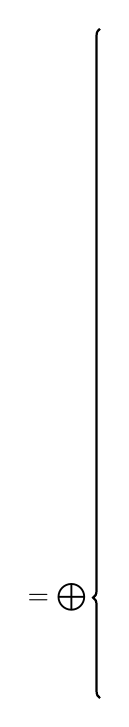
\begin{tikzpicture}
    \draw[decorate,thick,decoration={brace,aspect=0.15}] (0,-8.5) -- (0,0);
    \node[anchor=east,inner sep=0mm] at (-0.15,-7.225) {$= \bigoplus$};
  \end{tikzpicture}%
  \hfill%
  \subcaptionbox{%
    Hierarchical not-a-knot B-splines
    $\basis{l',i'}^{p,\notaknot}$ ($l' \le l$, $i' \in \hiset{l'}$)
    and grid points $\gp{l',i'}$ \emph{(dots)}.%
  }[74mm]{%
    \includegraphics{hierarchicalBSpline_6}%
  }%
  \caption{%
    Univariate nodal and hierarchical cubic not-a-knot B-splines ($p = 3$)
    up to level $l = 3$.
    The nodal space $\ns{l}^{p,\notaknot}$,
    which coincides with the not-a-knot spline space $\naksplspace{l}{p}$,
    decomposes into the direct sum
    of the hierarchical subspaces $\hs{l'}^{p,\notaknot}$ ($l' \le l$).
    The knots of each level $l'$ are given by removing the
    first $\tfrac{p-1}{2}$ and last $\tfrac{p-1}{2}$
    inner points \emph{(crosses)}
    from the set of grid points $\gp{l',i'}$
    ($i' = 0, \dotsc, 2^{l'}$).%
  }%
  \label{fig:notAKnotBSpline}%
\end{figure}

The motivation for using Lagrange polynomials for coarse levels
is that they form a basis of the polynomial space
and that they can be implemented and calculated quickly.
However, the specific choice of basis functions for the levels
$l < \lceil\log_2(p + 1)\rceil$ is arbitrary,
as long as these functions are linearly independent
(of each other and of the ``true'' not-a-knot B-splines
$\basis{l,i}^{p,\notaknot}$, $l \ge \lceil\log_2(p+1)\rceil$)
and contained in the space $\naksplspace{l}{p}$.

\paragraph{Implementation}

Note that in each level $l \ge \lceil\log_2(p+1)\rceil$,
only the first $\tfrac{p+1}{2}$
(indices $i = 1, 3, \dotsc, p$)
and the last $\tfrac{p+1}{2}$
(indices $i = 2^l - p, 2^l - p + 2, \dotsc, 2^l - 1$)
hierarchical basis functions $\basis{l,i}^{p,\notaknot}$
differ from $\basis{l,i}^p$,
i.e., we have
\begin{equation}
  \basis{l,i}^{p,\notaknot} = \basis{l,i}^p,\quad
  i = p + 2,\; p + 4,\; \dotsc,\; 2^l - p - 2.
\end{equation}
This means that we can reuse uniform B-spline code
for the inner functions.
Due to $\basis{l,i}^{p,\notaknot}(x) = \basis{l,2^l-i}^{p,\notaknot}(1-x)$
(because of the symmetry of $\nodalknotseq{l}{p}{\notaknot}$),
we only have to implement $\tfrac{p+1}{2}$ not-a-knot B-splines per level $l$.
As $\basis{l,i}^{p,\notaknot}$ and $\basis{l+1,i}^{p,\notaknot}$
use the same knots up to an affine transformation for $l$ large enough
($l \ge 3$ suffices for $p = 3$),
we only have to implement a number of special case for coarse levels $l$.
In other words, the not-a-knot approach is ``minimally invasive''
with respect to an implementation that already uses uniform B-splines.

\paragraph{Hierarchical splitting}

The main benefit of the hierarchical not-a-knot B-spline basis
is the validity of the hierarchical splitting.
Again usual, we define $\ns{l}^{p,\notaknot}$ and $\hs{l}^{p,\notaknot}$
as the nodal and the hierarchical not-a-knot subspace of level $l$,
respectively.

\begin{proposition}[hierarchical splitting for not-a-knot B-splines]
  \label{prop:hierSplittingNAKBSplineUV}
  \newgsymbol{Pp}{$P^p$}{%
    Space of all polynomials of degree $\le p$ on $\clint{0, 1}$%
  }%
  The hierarchical splitting \eqref{eq:hierSplittingUV}
  holds for the hierarchical not-a-knot B-spline basis:
  \begin{equation}
    \naksplspace{l}{p}
    = \ns{l}^{p,\notaknot}
    = \bigoplus_{l'=0}^l \hs{l'}^{p,\notaknot},
  \end{equation}
  where for $l < \lceil\log_2(p+1)\rceil$, $\naksplspace{l}{p}$
  is defined as the space $P^{2^l + 1}$ of polynomials of degree
  $\le 2^l + 1$ on $\clint{0, 1}$
  (for $l \ge \lceil\log_2(p+1)\rceil$,
  $\naksplspace{l}{p}$ is the not-a-knot spline space).
\end{proposition}

\begin{proof}
  For $l < \lceil\log_2(p+1)\rceil$, all
  three spaces coincide with $P^{2^l + 1}$ and nothing is to prove.
  
  For $l \ge \lceil\log_2(p+1)\rceil$,
  we check the two conditions of \thmref{lemma:hierSplittingUV}.
  First, the hierarchical subspace $\hs{l'}^{p,\notaknot}$ ($l' \le l$)
  is a subspace of $\naksplspace{l}{p} = \ns{l}^{p,\notaknot}$.
  This is a conclusion of \thmref{prop:splineSpace}, as
  every function $\basis{l',i'}^{p,\notaknot}$ ($i' \in \hiset{l'}$)
  is continuous on $\clint{0, 1}$, a polynomial on every knot interval of
  $\nodalknotseq{l}{p}{\notaknot}$, and at the knots themselves
  at least $(p - 1)$ times continuously differentiable.
  
  Second, the hierarchical functions $\basis{l',i'}^{p,\notaknot}$
  ($l' \le l$, $i' \in \hiset{l'}$) are linearly independent.
  This can be shown similar to the proof of
  \thmref{prop:hierBSplineLinearlyIndependent}.
  The linear independence of the Lagrange polynomials
  can be checked by inserting grid points into a zero linear combination.
  The linear combination collapses and only one term remains,
  the coefficient corresponding to the grid point.
  Hence, all coefficients must vanish.
\end{proof}

\begin{corollary}
  \label{cor:hierSplittingNAKBSplineMV}
  It holds
  \begin{equation}
    \naksplspace{\ßl}{\ßp}
    = \ns{\ßl}^{\ßp,\notaknot}
    = \bigoplus_{\ßl'=\ß0}^\ßl \hs{\ßl'}^{\ßp,\notaknot},
  \end{equation}
  where $\naksplspace{\ßl}{\ßp}$ is the
  tensor product space of $\naksplspace{l_t}{p_t}$
  ($t = 1, \dotsc, d$) as defined in \cref{prop:hierSplittingNAKBSplineUV}.
\end{corollary}

\begin{proof}
  Follows directly from \thmref{prop:splittingUVToMV}.
\end{proof}

\paragraph{Sparse grids with not-a-knot B-splines}

Regular sparse grid spaces using the new hierarchical not-a-knot basis
are defined analogously to the uniform case, i.e.,
\begin{equation}
  \label{eq:sparseGridRegularNAK}
  \regsgspace{n}{d}{\ßp,\notaknot}
  := \bigoplus_{\normone{\ßl} \le n} \hs{\ßl}^{\ßp,\notaknot}.
\end{equation}
\newgsymbol{Pp!}{$P^\ßp$}{%
  Space of all $d$-variate polynomials of
  coordinate degree $\le \ßp$ on $\clint{\ß0, \ß1}$%
}%
If the level $n$ is large enough, then $\regsgspace{n}{d}{\ßp,\notaknot}$
contains the space $P^\ßp$ of all $d$-variate polynomials of
coordinate degree $\le \ßp$ on $\clint{\ß0, \ß1}$
(i.e., functions $f\colon \clint{0, 1} \to \real$,
$f(\ßx) := \sum_{\ßq=\ß0}^\ßp \interpcoeff{\ßq} \prod_{t=1}^d x_t^{q_t}$,
with $\interpcoeff{\ßq} \in \real$).
This means that in contrast to the uniform B-spline basis,
hierarchical not-a-knot B-splines on sparse grids are able to exactly
represent global polynomials on $\clint{\ß0, \ß1}$:

\begin{corollary}
  If $n \ge \normone{\lceil\veclog_\ß2(\ßp + \ß1)\rceil}$,
  then $P^\ßp \subset \regsgspace{n}{d}{\ßp,\notaknot}$.
\end{corollary}

\begin{proof}
  Let $\ßl := \lceil\veclog_\ß2(\ßp + \ß1)\rceil$ and $n \ge \normone{\ßl}$.
  By \cref{cor:hierSplittingNAKBSplineMV}, we have
  $\bigoplus_{\ßl' \le \ßl} \hs{\ßl}^{\ßp,\notaknot} = \naksplspace{\ßl}{\ßp}$.
  In addition, all $\ßl' \in \natz^d$ with $\ßl' \le \ßl$ satisfy
  $\normone{\ßl'} \le n$ and thus,
  $\bigoplus_{\ßl' \le \ßl} \hs{\ßl}^{\ßp,\notaknot} \subset
  \regsgspace{n}{d}{\ßp,\notaknot}$ by \eqref{eq:sparseGridRegularNAK}.
  We conclude
  $P^\ßp \subset \naksplspace{\ßl}{\ßp} \subset
  \regsgspace{n}{d}{\ßp,\notaknot}$, which is the asserted claim.
\end{proof}



\subsection{Modified and Non-Uniform Hierarchical Not-A-Knot B-Splines}
\label{sec:323modifiedNAKBSplines}

\paragraph{Modified hierarchical not-a-knot B-splines}

Similar to uniform and Clenshaw--Curtis B-splines
(\cref{sec:31standardBSplines}),
it is possible to define a modified version of the
hierarchical not-a-knot B-spline basis to obtain
``reasonable'' boundary values without boundary points.
However, we cannot use \thmref{lemma:marsden} similarly to
\eqref{eq:modifiedBSplineConstruction}:
Due to the removal of knots, there is only a single
not-a-knot B-spline $\basis{l,0}^{p,\notaknot}$ left of
$\basis{l,1}^{p,\notaknot}$.
B-splines $\basis{l,i}^{p,\notaknot}$ with index $i < 0$
would be zero in $\clint{0, 1}$.

While we are therefore not able to construct modified functions
whose second derivative vanishes in neighborhood of $x = 0$,
we can at least use $\basis{l,0}^{p,\notaknot}$ to let the
second derivative vanish in $x = 0$ itself:
\begin{equation}
  \label{eq:modifiedNotAKnotBSpline}
  \basis{l,i}^{p,\modified,\notaknot}(x)
  :=
  \begin{cases}
    1,&
    l = 1,\quad i = 1,\\
    \basis{l,1}^{p,\notaknot}(x)
    - \basis{l,0}^{p,\notaknot}(x)
    \dfrac{\frac{\diff^2}{\dx^2} \basis{l,1}^{p,\notaknot}(0)}%
    {\frac{\diff^2}{\dx^2} \basis{l,0}^{p,\notaknot}(0)},&
    l \ge 2,\quad i = 1,\\
    \basis{l,i}^{p,\notaknot}(x),&
    l \ge 2,\quad i \in \hiset{l} \setminus \{1, 2^l - 1\},\\
    \basis{l,1}^{p,\modified,\notaknot}(1 - x),&
    l \ge 2,\quad i = 2^l - 1.
  \end{cases}
  \hspace*{-2mm}
\end{equation}
The resulting modified hierarchical Clenshaw--Curtis not-a-knot B-spline basis
$\basis{l,i}^{p,\modified,\notaknot}$ is shown with dashed lines
in \cref{fig:modifiedNotAKnotBSpline}.
As before, we have to implement $\basis{l,1}^{p,\modified,\notaknot}$
only for a single level $l$, as modified functions of higher levels
are the same up to an affine parameter transformation.
Note again that for $p \ge 5$, we would have to modify additional
interior B-splines as the interior of their support then extends to the
boundary of $\clint{0, 1}$.
We refrain from doing so to keep the definition
\eqref{eq:modifiedNotAKnotBSpline} simple.

\paragraph{Non-uniform hierarchical not-a-knot B-splines}

The not-a-knot construction is completely independent from the
distribution of the grid points at hand.
Consequently, we can define hierarchical not-a-knot B-splines
for non-uniform distributions.
For instance, to define not-a-knot B-splines for the
Chebyshev points in \cref{sec:314nonUniform},
we first specify the knot sequence as
\begin{subequations}
  \begin{gather}
    \nodalknotseq{l}{p}{\clenshawcurtis,\notaknot}
    := (\nodalknot{l,0}{p}{\clenshawcurtis,\notaknot}, \dotsc,
    \nodalknot{l,m+p}{p}{\clenshawcurtis,\notaknot}),\quad
    m := 2^l + 1,\\
    \nodalknot{l,k}{p}{\clenshawcurtis,\notaknot}
    :=
    \begin{cases}
      \gp{l,k-p}^\clenshawcurtis,&
      k = 0, \dotsc, p,\\
      \gp{l,k-(p+1)/2}^\clenshawcurtis,&
      k = p + 1, \dotsc, 2^l,\\
      \gp{l,k-1}^\clenshawcurtis,&
      k = 2^l + 1, \dotsc, 2^l + p + 1,
    \end{cases}
  \end{gather}
\end{subequations}
and then define hierarchical not-a-knot Clenshaw--Curtis B-splines as
\begin{subequations}
  \begin{gather}
    \basis{l,i}^{p,\clenshawcurtis,\notaknot}
    :=
    \begin{cases}
      L_{l,i}^\clenshawcurtis,&
      l < \lceil\log_2(p+1)\rceil,\\
      \nonunifbspl{i,\nodalknotseq{l}{p}{\clenshawcurtis,\notaknot}}{p},&
      l \ge \lceil\log_2(p+1)\rceil,
    \end{cases}\quad
    l \in \natz,\quad
    i \in \hiset{l},\\
    L_{l,i}^\clenshawcurtis\colon \clint{0, 1} \to \real,\quad
    L_{l,i}^\clenshawcurtis(x)
    := \prod_{\substack{i'=0,\dotsc,2^l\\i'\not=i}}
    \frac{x - \gp{l,i'}^\clenshawcurtis}%
    {\gp{l,i}^\clenshawcurtis - \gp{l,i'}^\clenshawcurtis}.
  \end{gather}
\end{subequations}
This definition can even be combined with modification
of hierarchical not-a-knot B-splines as discussed above.
We can use exactly the same approach as in
\eqref{eq:modifiedNotAKnotBSpline}, if we replace the
not-a-knot basis functions with their non-uniform not-a-knot counterparts
(not-a-knot Clenshaw--Curtis B-splines in the above example).
The hierarchical not-a-knot Clenshaw--Curtis B-spline basis of
cubic degree and the corresponding modified functions are plotted in
\cref{fig:clenshawCurtisNotAKnotBSpline}.

\begin{figure}
  \subcaptionbox{%
    $\basis{l',i'}^{p,\notaknot}$,
    $\basis{l',i'}^{p,\modified,\notaknot}$
    \emph{(dashed)}, and $\gp{l',i'}$ \emph{(dots)}.%
    \label{fig:modifiedNotAKnotBSpline}%
  }[73mm]{%
    \includegraphics{hierarchicalBSpline_7}%
  }%
  \hfill
  \subcaptionbox{%
    $\basis{l',i'}^{p,\clenshawcurtis,\notaknot}$,
    $\basis{l',i'}^{p,\modified,\clenshawcurtis,\notaknot}$
    \emph{(dashed)}, and $\gp{l',i'}^\clenshawcurtis$ \emph{(dots)}.%
    \label{fig:clenshawCurtisNotAKnotBSpline}%
  }[76mm]{%
    \includegraphics{hierarchicalBSpline_8}%
  }%
  \caption{%
    Comparison of hierarchical uniform and Clenshaw--Curtis cubic not-a-knot
    B-splines $\basis{l',i'}^{p,\notaknot}$ and
    $\basis{l',i'}^{p,\clenshawcurtis,\notaknot}$
    ($l ' \le l$, $i' \in \hiset{l'}$, $p = 3$) up to level $l = 3$
    together with the respective modified versions
    $\basis{l',i'}^{p,\modified,\notaknot}$ and
    $\basis{l',i'}^{p,\modified,\clenshawcurtis,\notaknot}$
    \emph{(dashed)}.
    The knots of each level $l'$ are given by removing the
    first $\tfrac{p-1}{2}$ and last $\tfrac{p-1}{2}$
    inner points \emph{(crosses)}
    from the set of grid points $\gp{l',i'}$ or
    $\gp{l',i'}^\clenshawcurtis$
    ($i' = 0, \dotsc, 2^{l'}$), respectively.%
  }%
\end{figure}



\subsection{Other Approaches to Incorporate Boundary Conditions}
\label{sec:324naturalBoundary}

Not-a-knot boundary conditions are not the only approach
to obtain a subspace of $\wholesplspace{l}{p}$ with the right dimension $2^l - 1$.
Another possibility, which we want to discuss briefly, are
\term{natural boundary conditions}.
In the cubic case, for which they are usually formulated
\cite{Hoellig13Approximation},
these boundary conditions require that the
second derivatives $\frac{\diff^2}{\dx^2} \basis{l,i}$ of the
basis functions vanish at the boundary $x \in \{0, 1\}$.
To obtain the necessary number of $p - 1$ constraints also
for higher degrees $p$,
we require that all derivatives
$\frac{\diff^q}{\dx^q} \basis{l,i}$ of order
$q = 2, \dotsc, \tfrac{p+1}{2}$ vanish at $x \in \{0, 1\}$.

\newgsymbol{.nat}{$\cdot^\ntrl$}{%
  Superscript for ``Natural (basis
  function/function space/interpolant)''%
}%
Consequently, we can define hierarchical natural B-splines as
\begin{subequations}
  \begin{gather}
    \basis{l,i}^{p,\ntrl}(x)
    :=
    \begin{cases}
      L_{0,i}(x),&
      l = 0,\\
      \basis{l,i}^p +
      \sum_{j \in J_i^{p,\ntrl}} c_{l,i,j} \basis{l,j}^p,&
      l \ge 1,
    \end{cases}\quad
    l \in \natz,\quad
    i \in \hiset{l},\\
    J_i^{p,\ntrl}
    := \{i+1-\tfrac{p+1}{2}, \dotsc, i-1\} \cup
    \{i+1, \dotsc, i-1+\tfrac{p+1}{2}\},
  \end{gather}
\end{subequations}
where the coefficients $c_{l,i,j} \in \real$ are chosen such that
the natural boundary conditions are satisfied:
\begin{equation}
  \frac{\diff^q}{\dx^q} \basis{l,i}^{p,\ntrl}(x)
  = 0,\quad
  l \ge 1,\quad
  i \in \hiset{l},\quad
  q = 2, \dotsc, \tfrac{p+1}{2},\quad
  x \in \{0, 1\}.
\end{equation}
Note that the first half of the coefficients $c_{l,i,j} \in \real$
($j < i$) vanish if the interior of the support of $\basis{l,i}^p$
does not contain $x = 0$
(i.e., $i > \tfrac{p+1}{2}$).
The second half of the coefficients~($j > i$) vanishes analogously
if $1 \notin \interiorsupp \basis{l,i}^p \iff i < 2^l - \tfrac{p+1}{2}$.
This means that as for the not-a-knot basis,
only the first $\tfrac{p+1}{2}$ and the last $\tfrac{p+1}{2}$
hierarchical functions have to be altered in each level.

\Cref{fig:naturalBSpline} shows the hierarchical natural spline basis.
The main disadvantage of natural boundary conditions is that
we are not able to replicate arbitrary polynomials exactly on $\clint{0, 1}$
with this approach.
Only polynomials that satisfy natural boundary conditions themselves
(linear polynomials for example)
can be represented exactly with hierarchical natural B-splines.
For this reason, we do not further consider this basis in the
rest of the thesis.

\begin{SCfigure}
  \includegraphics{hierarchicalBSpline_9}%
  \caption{%
    Hierarchical cubic natural B-splines
    $\basis{l',i'}^{p,\ntrl}$
    ($l' \le l$, $i' \in \hiset{l'}$, $p = 3$) and
    grid points $\gp{l',i'}$ \emph{(dots)} up to level $l = 3$.%
  }%
  \label{fig:naturalBSpline}%
\end{SCfigure}


\cleardoublepage
